% Author: Rasmus Pank Roulund
\documentclass{standalone}
\usepackage{tikz}
\usetikzlibrary{shapes.geometric, arrows,positioning,calc,fit}

\begin{document}

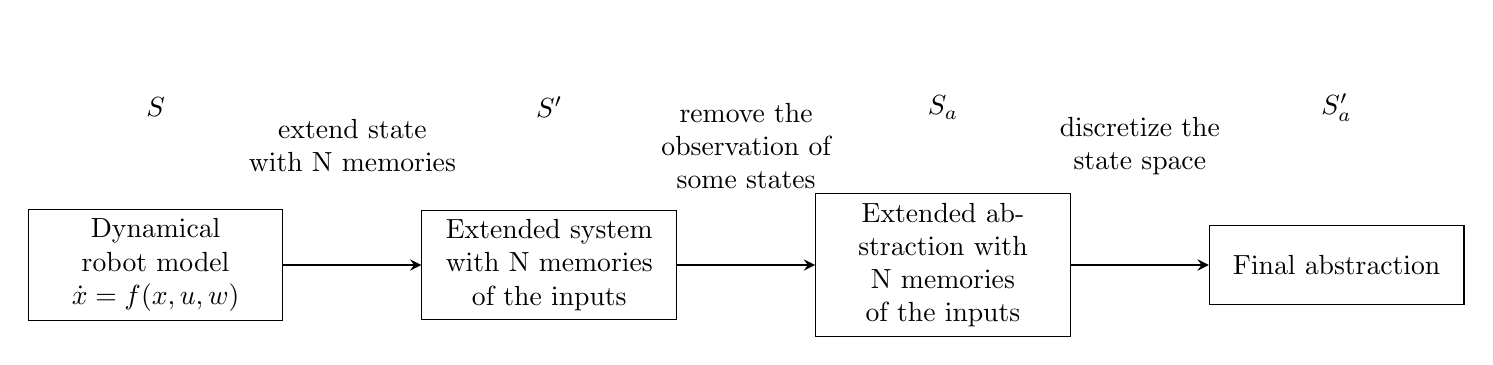
\begin{tikzpicture}[node distance = 2cm]

\tikzstyle{cell} = [rectangle, minimum width=3cm, minimum height=1cm,text centered, draw=black, text width=3cm,on grid,auto,xshift=3cm]
\tikzstyle{info} = [rectangle, minimum width=3cm, minimum height=3cm,text centered, draw=none, text width=3cm,on grid,auto,above]
\tikzstyle{labels} = [rectangle,text centered, draw=none,on grid,auto]
\tikzstyle{arrow} = [thick,->,>=stealth]

%% ------------------
%% -- OFFLINE PART --
%% ------------------

% FTS
\node (dyn_robot) 	[cell] {Dynamical robot model ${\dot{x} = f(x,u,w)}$};
\node (ext_sys) 			[cell, right of=dyn_robot] {Extended system with N memories of the inputs};
\node (ext_abstr) 			[cell, right of=ext_sys] {Extended abstraction with N memories of the inputs};
\node (abstr) 			[cell, right of=ext_abstr] {Final abstraction};

\node (s) 			[labels,above of=dyn_robot] {$S$};
\node (sp) 			[labels, above of=ext_sys] {$S'$};
\node (sa) 			[labels, above of=ext_abstr] {$S_a$};
\node (sap) 			[labels, above of=abstr] {$S_a'$};


\draw [arrow] (dyn_robot) -- node[info]{extend state with N memories} (ext_sys);
\draw [arrow] (ext_sys) -- node[info]{remove the observation of some states} (ext_abstr);
\draw [arrow] (ext_abstr) -- node[info]{discretize the state space} (abstr);



\end{tikzpicture}

\end{document}
